%
%
%
%
% Make this longer
%
%
%
%

% Uncomment this to make slides with overlays:
%\documentclass[slides]{beamer}

% Uncomment these (but comment the above \documentclass line) to make handouts:
\documentclass[handout]{beamer}

% Uncomment these to have more than one slide per page
\usepackage{pgfpages}
\pgfpagesuselayout{2 on 1}[border shrink=5mm]
\pgfpageslogicalpageoptions{1}{border code=\pgfusepath{stroke}}
\pgfpageslogicalpageoptions{2}{border code=\pgfusepath{stroke}}

\usepackage[]{graphicx, color, hyperref}

\mode<presentation>
{
	%\usetheme[secheader]{Boadilla}
	%\usecolortheme[rgb={.835, .102,.169}]{structure}  
	\usetheme[width= 0cm]{Goettingen}
	%\setbeamercovered{transparent}
}
\setbeamertemplate{navigation symbols}{}
\setbeamertemplate{footline}[frame number]

\definecolor{blue2}{rgb}{0.278,0.278,0.729} 
\newcommand{\blue}[1]{\textcolor{blue2}{#1}}
\newcommand{\white}[1]{\textcolor{white}{#1}}
\newcommand{\red}[1]{\textcolor{red}{#1}}
\newcommand{\xbar}{\overline{x}}
\newcommand{\ybar}{\overline{y}}
\newcommand{\phat}{\widehat{p}}
\newcommand{\prob}{\mbox{Pr}}
\newcommand{\E}{\mathbb{E}}
\newcommand{\Var}{\mbox{Var}}
\newcommand{\cp}{\oplus}
\newcommand{\cm}{\circleddash}

\title{Lecture 3: Observational Studies + Randomized Experiments + Confounding + Simpsons's Paradox}
\author{Chapter 1.4}
\date{}


\begin{document}
%------------------------------------------------------------------------------
\begin{frame}
\titlepage
\end{frame}
%------------------------------------------------------------------------------


%------------------------------------------------------------------------------
\begin{frame}
\frametitle{Goals for Today}

\begin{itemize}
\item We illustrate the difference between
\begin{itemize}
  \item an \blue{observational study}
  \item a \blue{randomized experiment}, where the treatment is assigned at random.
\end{itemize}
\item Introduce the notion of confounding AKA lurking variables
\item Discuss \blue{Simpson's Paradox} (not in textbook).
\end{itemize}

\end{frame}
%------------------------------------------------------------------------------


%------------------------------------------------------------------------------
\begin{frame}
\frametitle{Going Back to Previous Example}

Going back to the study on 
\begin{center}
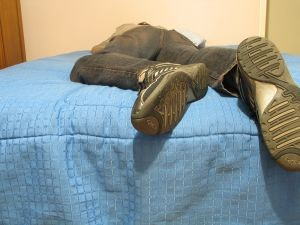
\includegraphics[width=0.3\textwidth]{figure/shoes.jpg}
\hspace{1cm}
$\Longrightarrow$
\hspace{1cm}
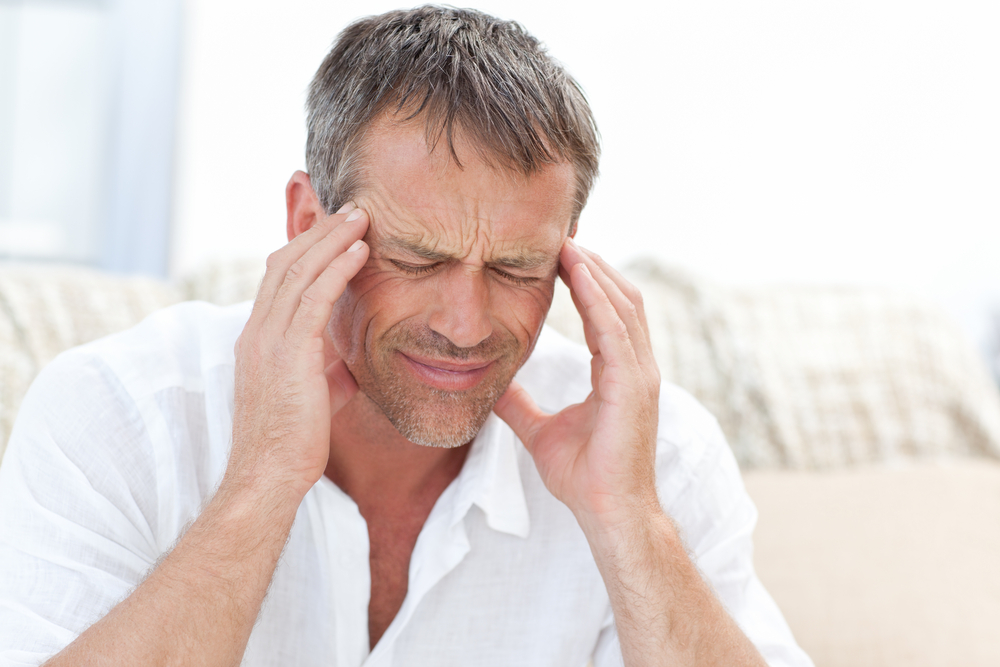
\includegraphics[width=0.3\textwidth]{figure/headache.jpg}
\end{center}

\begin{itemize}
\item The explanatory variable was: sleeping with your shoes on
\item The response variable was: waking up with a headache
\item The doctor hypothesized a \blue{causal} relationship
\end{itemize}

\end{frame}
%------------------------------------------------------------------------------


%------------------------------------------------------------------------------
\begin{frame}
\frametitle{Confounding Variable AKA Lurking Variable}

%
% Comment this
%
%This is an example of \blue{confounding}.  A confounding variable affects both the explanatory and response variable.  So if:
%
%\begin{itemize}
%\pause\item $x$ is the explanatory variable
%\pause\item $y$ is the response variable
%\pause\item $z$ is the confounding variable
%\end{itemize}
%we have:
%\vspace{6cm}

\end{frame}
%------------------------------------------------------------------------------


%------------------------------------------------------------------------------
\begin{frame}
\frametitle{Controlling for Potential Confounding}

%
% Comment this
%
%One way to \blue{control for} (i.e. take into account) confounding is to do an exhaustive search for all such variables.  This is not always practical.
%
%\vspace{0.25in}
%
%\pause Another way is via an experiment where we randomly assign individuals to a \blue{treatment} or a \blue{control} group in a \blue{randomized experiment}.  That way any differences in confounding variables between the two groups will even out in the long run.

\end{frame}
%------------------------------------------------------------------------------


%------------------------------------------------------------------------------
\begin{frame}
\frametitle{Back to Shoes and Headaches}

So imagine we recruit 10,000 people and \blue{randomly assign} 5000 to:

\begin{itemize}
\item the treatment group: sleep with shoes
\item the control group: sleep without shoes
\end{itemize}

\pause i.e.
\begin{center}
	\begin{tabular}{c|cc}
		Group & $n$ & \# with headache\\
		\hline	
		Treatment & 5000 & $n_1$\\
		Control & 5000 & $n_2$\\
  \end{tabular}
\end{center}
$n_1$ and $n_2$ won't be very different i.e. no difference in headache level regardless of shoes. 

\end{frame}
%------------------------------------------------------------------------------


%------------------------------------------------------------------------------
\begin{frame}
\frametitle{Observational Studies vs Randomized Experiments}

%
% Comment this.
%
%The key word from the study design above was \blue{randomly assign}.
%
%\begin{itemize}
%  \pause\item \blue{Observational studies}: a study where researchers have \blue{no control} over who receives the treatment
%  \pause\item \blue{Randomized experiments}: a study where researchers not only have control over who receives the treatment, but also make the assignments \blue{at random}.
%\end{itemize}

\end{frame}
%------------------------------------------------------------------------------


%------------------------------------------------------------------------------
\begin{frame}
\frametitle{Observational Studies vs Randomized Experiments}

The shoe/headache study introduced at the end of the last lecture is an \blue{observational study}, so we cannot conclude that wearing shoes when you sleep causes you wake up with a headache.

\end{frame}
%------------------------------------------------------------------------------


%------------------------------------------------------------------------------
\begin{frame}
\frametitle{Maxim of Statistics}

%
% Comment this
%
%\blue{Correlation is not causation}  Just because two variables appear to be associated/correlated, does not mean that one is \blue{causing the other}.

\pause \begin{itemize}
\item Spurious correlations:  \blue{\href{http://www.tylervigen.com/spurious-correlations}{http://www.tylervigen.com/}}
\item Saturday Morning Breakfast Cereal:  \blue{\href{http://www.smbc-comics.com/?id=3129}{http://www.smbc-comics.com/?id=3129}}
\end{itemize}



\end{frame}
%------------------------------------------------------------------------------




%------------------------------------------------------------------------------
\begin{frame}
\frametitle{Well-Known Example of Confounding}

A famous example of an unaccounted for confounding variable is UC Berkeley admissions data.  UCB was sued in 1973 for bias against women who had applied for admission to graduate schools. 

\vskip 0.5cm

\pause Let's consider the $n=4526$ people who applied to the 6 largest departments.

\end{frame}
%------------------------------------------------------------------------------



%------------------------------------------------------------------------------
\begin{frame}
\frametitle{Of the $n=4526$ applicants:}

\begin{center}
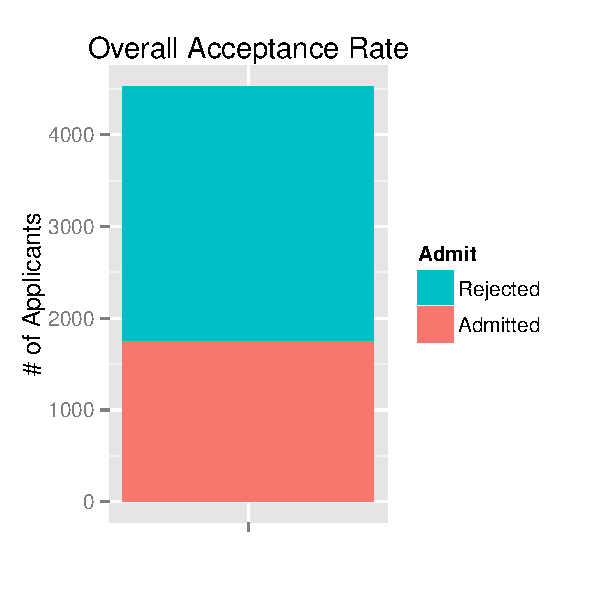
\includegraphics[height=\textheight]{figure/overall.pdf}
\end{center}

\end{frame}
%------------------------------------------------------------------------------



%------------------------------------------------------------------------------
\begin{frame}
\frametitle{Split the counts by gender:}

\begin{center}
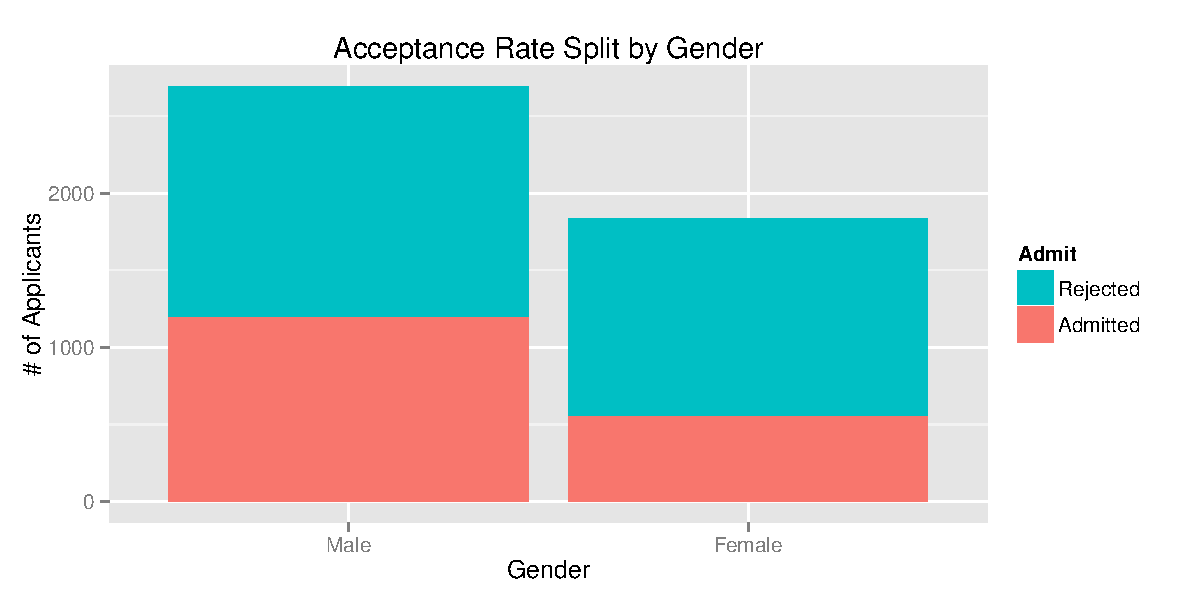
\includegraphics[width=\textwidth]{figure/gender-accpt-count.pdf}
\end{center}

\end{frame}
%------------------------------------------------------------------------------



%------------------------------------------------------------------------------
\begin{frame}
\frametitle{Look at proportions instead of counts:}

\begin{center}
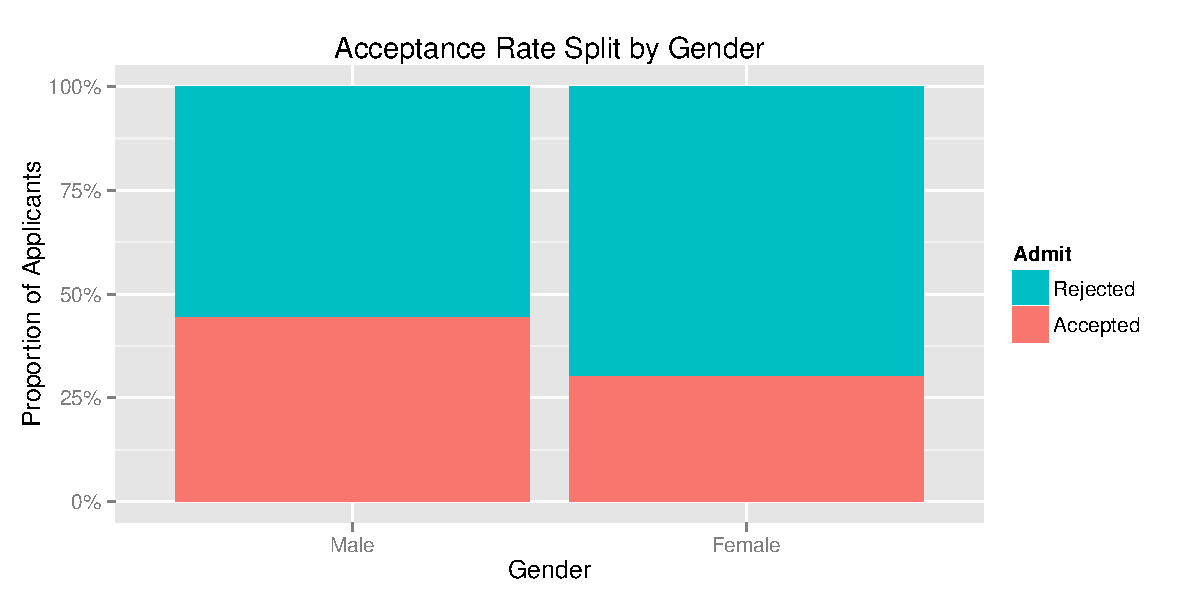
\includegraphics[width=\textwidth]{figure/gender-accpt.pdf}
\end{center}

\end{frame}
%------------------------------------------------------------------------------



%------------------------------------------------------------------------------
\begin{frame}
\frametitle{What was the ``competitiveness'' of departments?}

\begin{center}
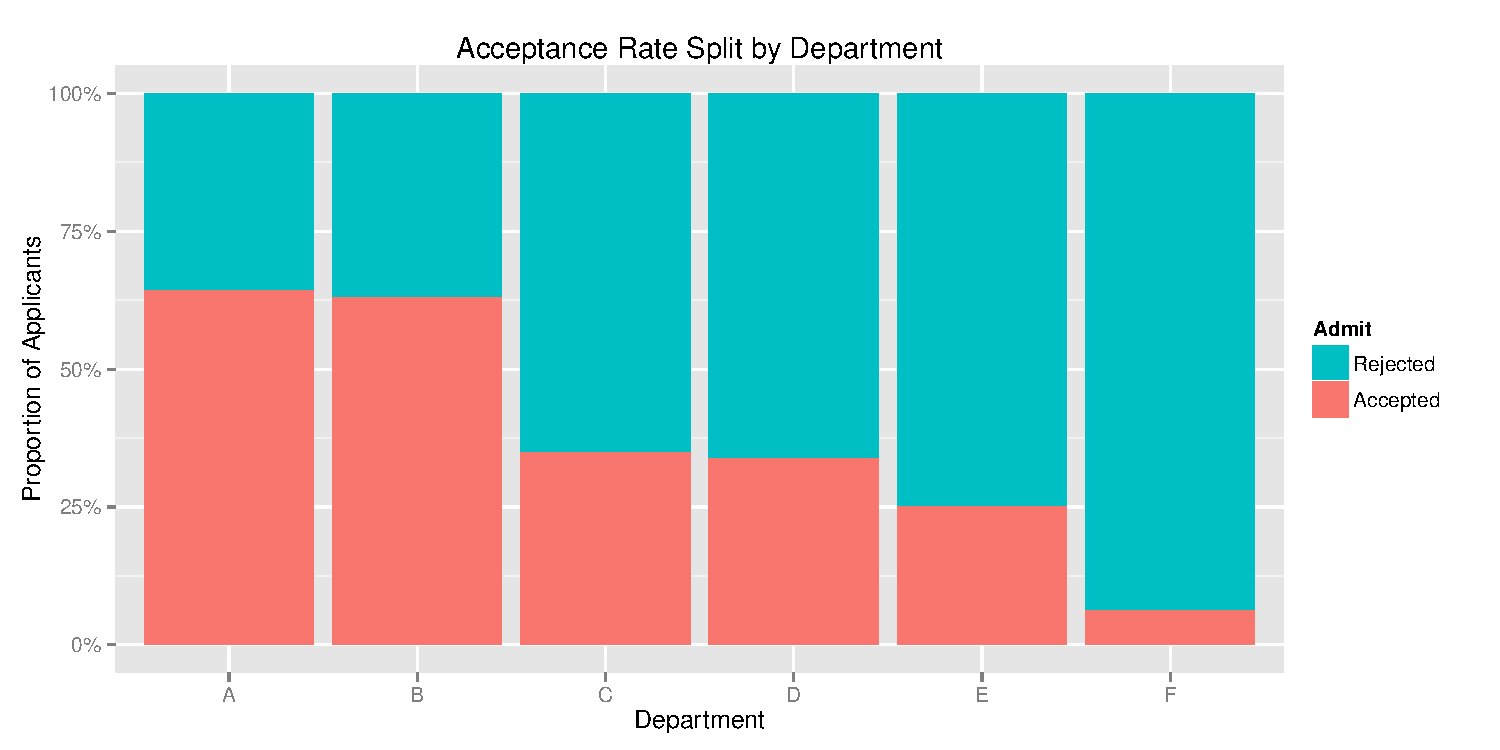
\includegraphics[width=\textwidth]{figure/dept-accpt.pdf}
\end{center}

\end{frame}
%------------------------------------------------------------------------------



%------------------------------------------------------------------------------
\begin{frame}
\frametitle{Where were the women applying?}

\begin{center}
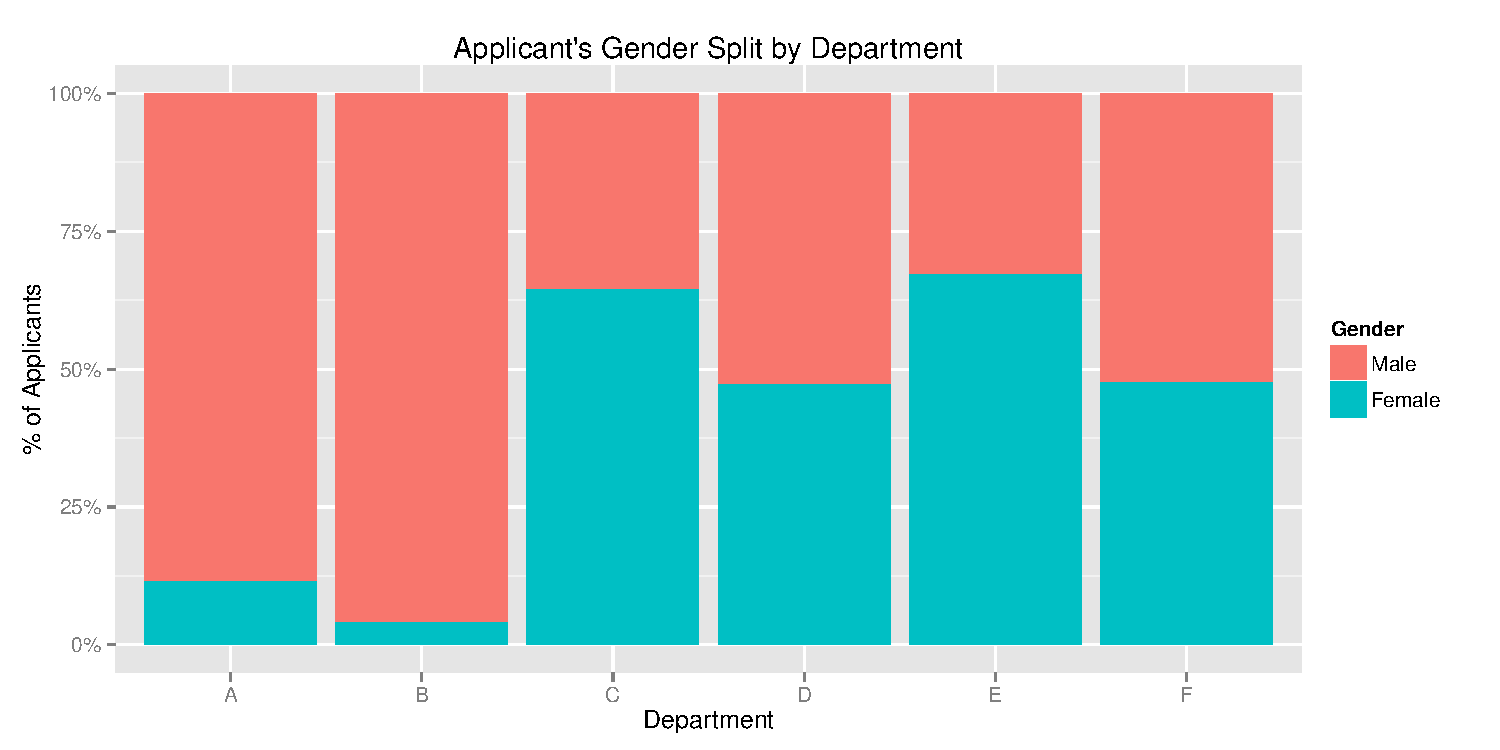
\includegraphics[width=\textwidth]{figure/dept-gender.pdf}
\end{center}

\end{frame}
%------------------------------------------------------------------------------



%------------------------------------------------------------------------------
\begin{frame}
\frametitle{So while in aggregate things looked like this:}

\begin{center}
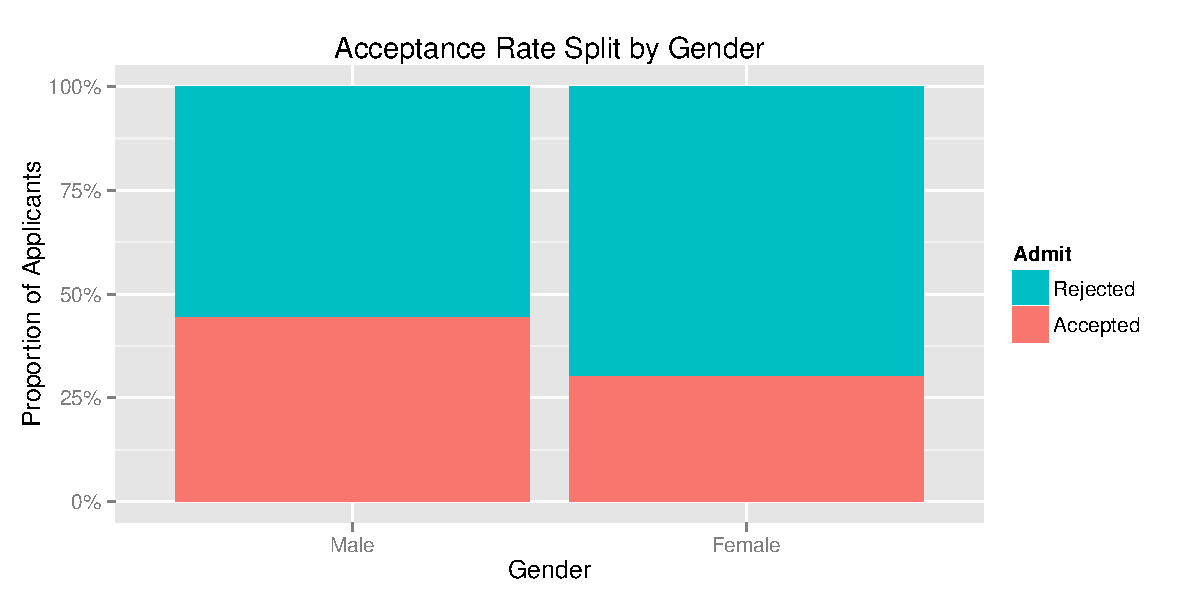
\includegraphics[width=\textwidth]{figure/gender-accpt.pdf}
\end{center}

\end{frame}
%------------------------------------------------------------------------------



%------------------------------------------------------------------------------
\begin{frame}
\frametitle{You need to account for department!}

\begin{center}
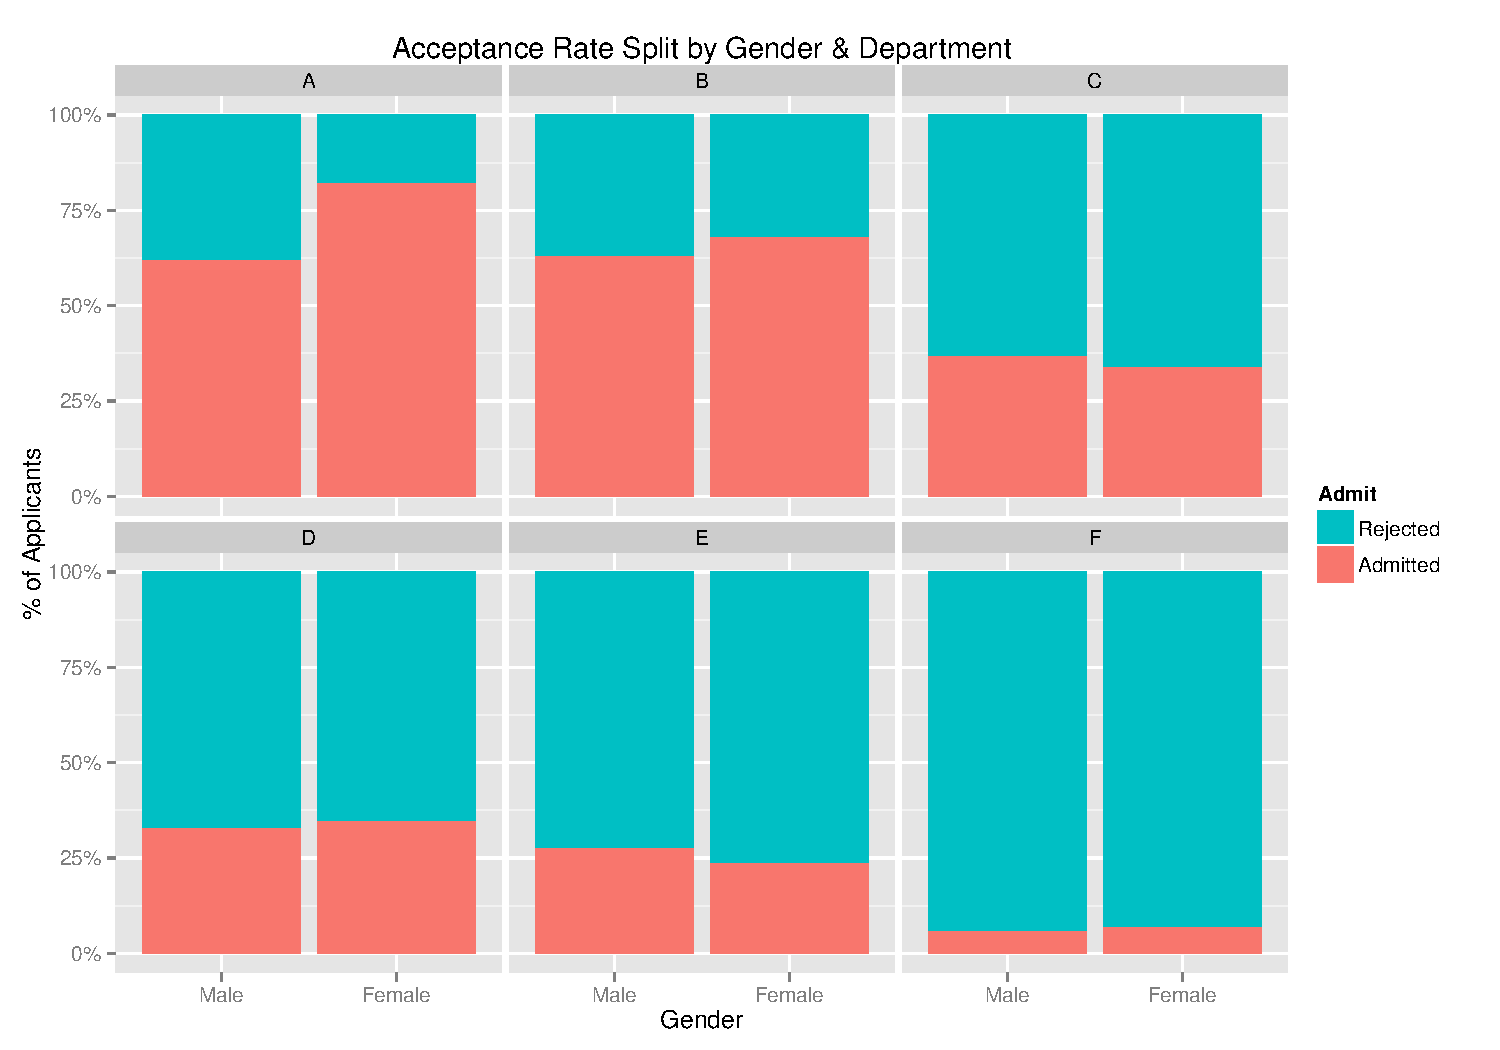
\includegraphics[width=\textwidth]{figure/split-accpt.pdf}
\end{center}

\end{frame}
%------------------------------------------------------------------------------


%------------------------------------------------------------------------------
\begin{frame}
\frametitle{Bickel et al.'s (1975) Explanation}

There was a confounding variable: \blue{competitiveness of department}, which is a function
\begin{itemize}
\item \# of applicants
\item \# of available slots
\end{itemize}

\vskip 0.5cm

\pause Departments weren't discriminating against women per se, rather:
\begin{itemize}
\pause \item women tended to apply to departments with high competition and hence lower admission rates, primarily the humanities.
\pause \item men tended to apply to departments with low competition and hence higher admission rates, primarily the sciences.
\end{itemize}

\end{frame}
%------------------------------------------------------------------------------


%------------------------------------------------------------------------------
\begin{frame}
\frametitle{Bickel et al.'s (1975) Explanation}

In fact, Bickel et al. found that ``If the data are properly pooled...there is a small but statistically significant bias in favor of women.''

\vskip 0.5cm

\pause This was the exact opposite claim of the lawsuit.  This is known as \blue{Simpson's Paradox}.  

\end{frame}
%------------------------------------------------------------------------------



%------------------------------------------------------------------------------
\begin{frame}
\frametitle{Simpson's Paradox}

%(From Wikipedia) Simpson's paradox occurs when a trend that appears in different groups of data disappears when these groups are combined, and the \blue{reverse trend} appears for the aggregate data.  
%
%\vspace{0.25in}
%
%\pause This is due to a confounding variable.

\end{frame}
%------------------------------------------------------------------------------



%------------------------------------------------------------------------------
\begin{frame}
\frametitle{A Graphical Illustration of Simpson's Paradox}
Say we have the following points: \textcolor{white}{lorem ipsum lorem ipsum lorem ipsum lorem ipsum}
\begin{center}
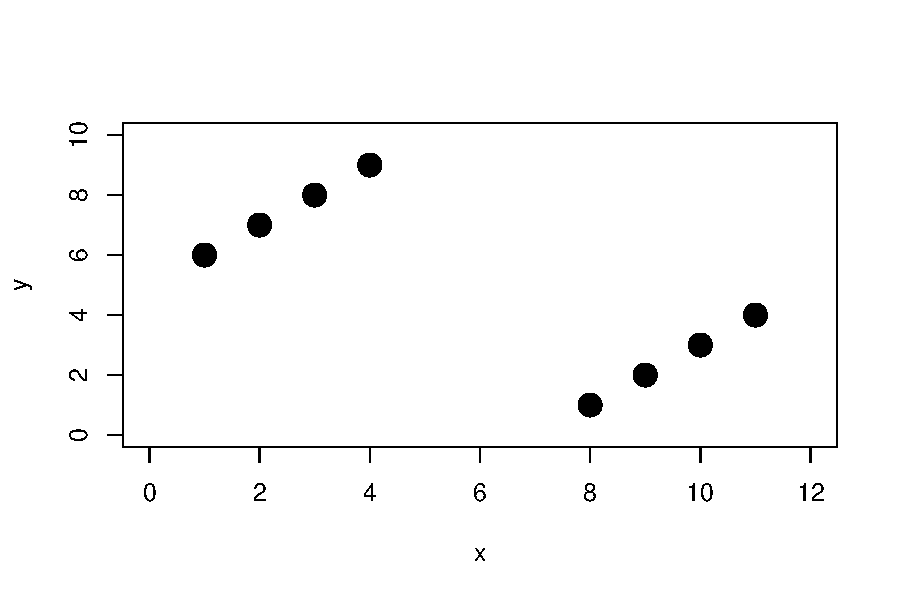
\includegraphics[width=10cm]{figure/simpsons1.pdf}
\end{center}

\end{frame}
%------------------------------------------------------------------------------



%------------------------------------------------------------------------------
\begin{frame}
\frametitle{A Graphical Illustration of Simpson's Paradox}
Overall, the best fitting single line suggests $x$ is \blue{negatively} related with $y$:
\begin{center}
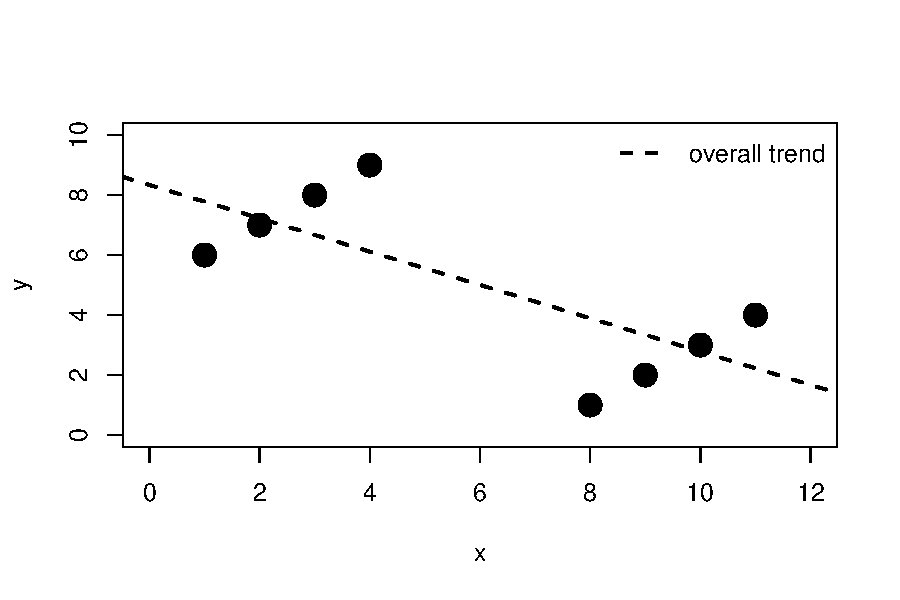
\includegraphics[width=10cm]{figure/simpsons2.pdf}
\end{center}

\end{frame}
%------------------------------------------------------------------------------



%------------------------------------------------------------------------------
\begin{frame}
\frametitle{A Graphical Illustration of Simpson's Paradox}
But say we have the \blue{confounding} variable color and fit two separate lines for each group: \textcolor{white}{lorem ipsum lorem ipsum}
\begin{center}
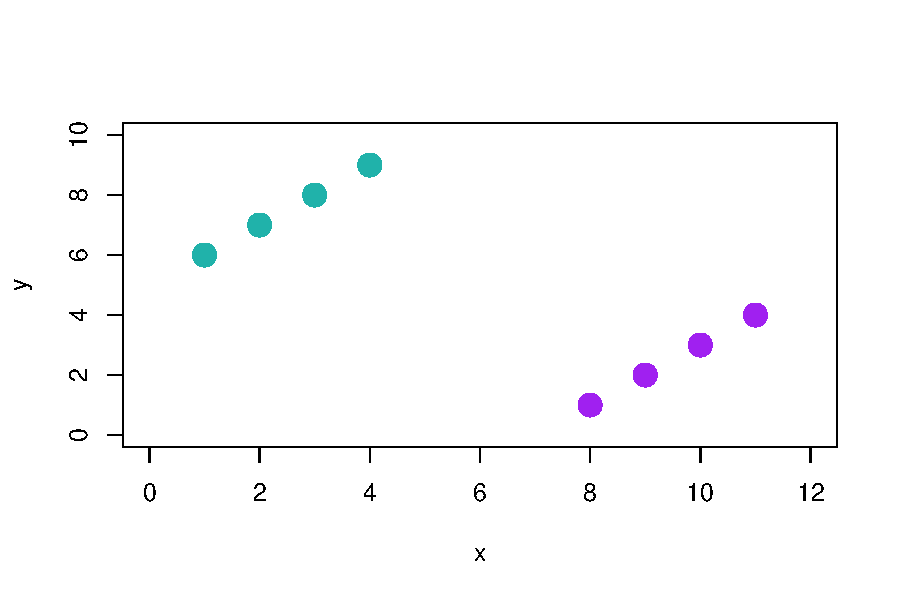
\includegraphics[width=10cm]{figure/simpsons3.pdf}
\end{center}

\end{frame}
%------------------------------------------------------------------------------



%------------------------------------------------------------------------------
\begin{frame}
\frametitle{A Graphical Illustration of Simpson's Paradox}
The subgroups now exhibit a \blue{positive} relationship! \textcolor{white}{lorem ipsum lorem ipsum}
\begin{center}
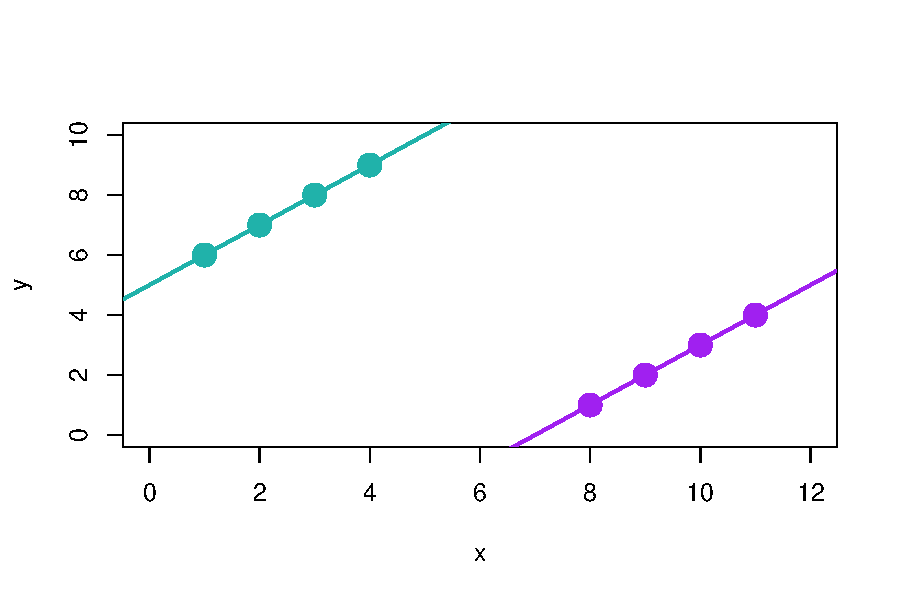
\includegraphics[width=10cm]{figure/simpsons4.pdf}
\end{center}

\end{frame}
%------------------------------------------------------------------------------



%------------------------------------------------------------------------------
\begin{frame}
\frametitle{A Graphical Illustration of Simpson's Paradox}
i.e. the trend in aggregate is the \blue{reverse} of the trend in the subgroups (teal \& purple).
\begin{center}
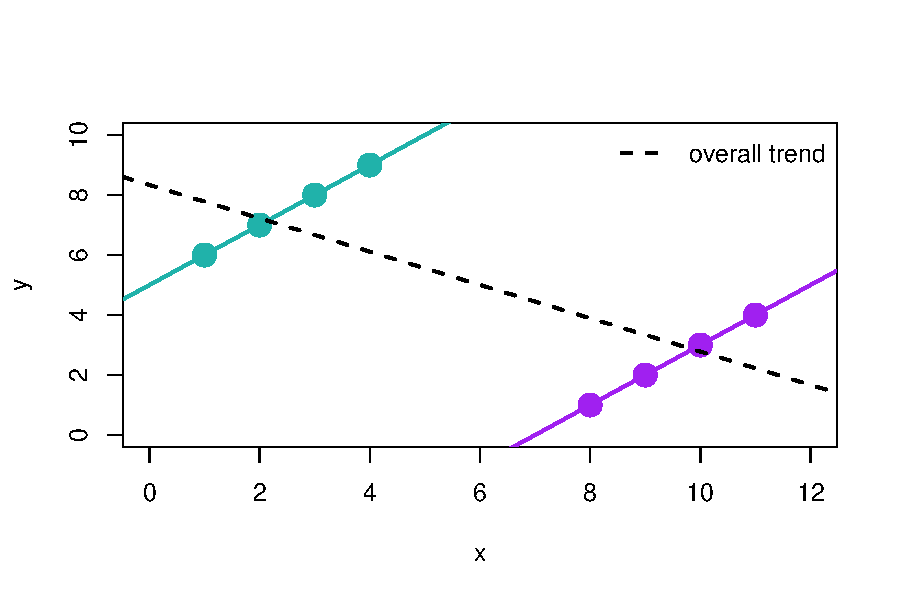
\includegraphics[width=10cm]{figure/simpsons5.pdf}
\end{center}

\end{frame}
%------------------------------------------------------------------------------



%------------------------------------------------------------------------------
\begin{frame}
\frametitle{Bickel et al.'s (1975) Conclusion}

``The bias in the aggregated data stems not from any pattern of discrimination on the part of admissions committees, which seem quite fair on the whole, \pause but apparently from prior screening at earlier levels of the educational system.''

\vspace{0.25in}

\pause ``Women are shunted by their socialization and education toward fields of graduate study that are generally more crowded, less productive of completed degrees, and less well funded, and that frequently offer poorer professional employment prospects.''

\vspace{0.25in}

The original paper can be found \blue{\href{http://www.unc.edu/~nielsen/soci708/cdocs/Berkeley\_admissions\_bias.pdf}{here}}.

\end{frame}
%------------------------------------------------------------------------------



%------------------------------------------------------------------------------
\begin{frame}
\frametitle{Next time}

We will discuss 
\begin{itemize}
\item Specific types of sampling beyond just \blue{simple random sampling}, as this is not always feasible
\pause\item Experimental design:  some key principles to keep in mind when evaluating the efficacy of treatments. 
\end{itemize}

\end{frame}
%------------------------------------------------------------------------------



\end{document}
























%%------------------------------------------------------------------------------
%\begin{frame}
%\frametitle{Statistics in Society: Civil Rights Act}
%
%From an \href{http://www.theguardian.com/commentisfree/2013/aug/28/republicans-party-of-civil-rights}{\blue{article}} in The Guardian on 2013/8/13 ``Were Republicans really the party of civil rights in the 1960s?''
%
%\begin{quotation}
%Some like to point out that the (Republican) party has a long history of standing up for civil rights compared to Democrats. Democrats, for example, were less likely to vote for the civil rights bills of the 1950s and 1960s. Democrats were more likely to filibuster...
%
%\vspace{0.25cm}
%
%Let's use the 1964 Civil Rights Act as our focal point. It was arguably the most important of the many civil rights bills passed in the middle part of the 20th century. It outlawed many types of racial and sexual discrimination, including access to hotels, restaurants, and theaters. In the words of Vice President Biden, it was a big ``f-ing deal''.
%\end{quotation}
%\end{frame}
%%------------------------------------------------------------------------------
%
%
%%------------------------------------------------------------------------------
%\begin{frame}
%\frametitle{Statistics in Society: Civil Rights Act}
%
%Let's investigate the Republican claim using the vote breakdown in the House of Representatives, split by both the representative's
%\begin{itemize}
%\item party affiliation: Repub or Dem
%\item home state: whether or not it was part of the Union or the Confederacy during the American Civil War
%\end{itemize}
%
%\end{frame}
%%------------------------------------------------------------------------------
%
%
%%------------------------------------------------------------------------------
%\begin{frame}
%\frametitle{Civil Rights Act Vote Breakdown}
%
%\begin{center}
%	\begin{tabular}{c|ccc|ccc}
%     & \multicolumn{3}{c|}{Democrats}  & \multicolumn{3}{c}{Republicans} \\ 
%     & Pro & Total & \% & Pro & Total & \% \\ 
%     \hline
%     
\includegraphics[height=0.4cm]{conf} & 8 & \textcolor{red}{91} & \blue{8\%} & 0 & \textcolor{red}{11} & 0\% \\ 
%	 
\includegraphics[height=0.4cm]{union} & 144 & \textcolor{red}{152} & \blue{95\%} & 137 & \textcolor{red}{161} & 85\% \\ 
%    \hline
%     Total & 152 & 243 & 62\% & 137 & 172 & \blue{80\%} \\ 
%  \end{tabular}
%\end{center}
%
%We observe that 
%\begin{enumerate}
%\item \textcolor{red}{91/(91 + 152) = 37\%} of Democrats
%\item \textcolor{red}{11/(11+161) = 6\%} of Republicans
%\end{enumerate}
%were from former confederate states.
%
%\end{frame}
%%------------------------------------------------------------------------------
%
%
%%------------------------------------------------------------------------------
%\begin{frame}
%\frametitle{Confederate vs Union States}
%
%This is not a fair comparison between Dems and Repubs!  Why?
%
%\vspace{0.25cm}
%
%\begin{center}
%	\begin{tabular}{c|ccc|ccc}
%     & \multicolumn{3}{c|}{
\includegraphics[height=0.4cm]{conf}}  & \multicolumn{3}{c}{
\includegraphics[height=0.4cm]{union}} \\ 
%     & Pro & Total & \% & Pro & Total & \% \\ 
%    \hline
%     Total & 8 & 102 & 8\% & 281 & 313 & \blue{90\%} \\ 
%     \multicolumn{7}{c}{}
%  \end{tabular}
%\end{center}
%
%\vspace{0.1cm}
%
%There is an enormous difference in support for the Civil Rights Act between Confederate and Union states!
%
%\end{frame}
%%------------------------------------------------------------------------------
%
%
%%------------------------------------------------------------------------------
%\begin{frame}
%\frametitle{Not a Fair Comparison}
%So...
%
%\begin{center}
%	\begin{tabular}{c|ccc|ccc}
%     & \multicolumn{3}{c|}{Democrats}  & \multicolumn{3}{c}{Republicans} \\ 
%     & Pro & Total & \% & Pro & Total & \% \\ 
%     \hline
%     
\includegraphics[height=0.4cm]{conf} & 8 & \textcolor{red}{91} & \blue{8\%} & 0 & \textcolor{red}{11} & 0\% \\ 
%	 
\includegraphics[height=0.4cm]{union} & 144 & \textcolor{red}{152} & \blue{95\%} & 137 & \textcolor{red}{161} & 85\% \\ 
%    \hline
%     Total & 152 & 243 & 62\% & 137 & 172 & \blue{80\%} \\ 
%  \end{tabular}
%\end{center}
%is not an apples to apples comparison!  We need to level the playing field.
%
%\end{frame}
%%------------------------------------------------------------------------------
%
%
%%------------------------------------------------------------------------------
%\begin{frame}
%\frametitle{Leveling the Playing Field}
%\begin{small}
%So let's imagine a hypothetical world of Repubs where
%\begin{enumerate}
%\item we have the same number of Repubs (172)
%\item the Repub voting percentages stay the same (0\% and 85\%)
%\item CRUCIAL: the Confederate/Union mix is the same as with the Dems (\textcolor{red}{91 vs 152} i.e. 37\% vs 63\%) 
%\end{enumerate}
%\end{small}
%
%
%\begin{center}
%	\begin{tabular}{c|ccc|ccc}
%     & \multicolumn{3}{c|}{Democrats}  & \multicolumn{3}{c}{Republicans} \\ 
%     & Pro & Total & \% & Pro & Total & \% \\ 
%     \hline
%     
\includegraphics[height=0.4cm]{conf} & 8 & \textcolor{red}{91} & \blue{8\%} & 0 & 64 & 0\% \\ 
%	 
\includegraphics[height=0.4cm]{union} & 144 & \textcolor{red}{152} & \blue{95\%} & 92 & 108 & 85\% \\ 
%    \hline
%     Total & 152 & 243 & \blue{62\%} & 92 & 172 & 53\% \\ 
%  \end{tabular}
%\end{center}
%
%\begin{enumerate}
%\item 37\% $\times$ 172 = 64
%\item 172 - 64 = 108
%\item 64 $\times$ 0\% = 0 and 108 $\times$ 85\% = 92
%\item 92/(92+172) = 53\%
%\end{enumerate}
%
%\end{frame}
%%------------------------------------------------------------------------------
%
%
%%------------------------------------------------------------------------------
%\begin{frame}
%\frametitle{Summary}
%
%\blue{Real data}: different Confederate/Union proportions between Dems/Repubs
%\begin{center}
%	\begin{tabular}{c|ccc|ccc}
%     & \multicolumn{3}{c|}{Democrats}  & \multicolumn{3}{c}{Republicans} \\ 
%     & Pro & Total & \% & Pro & Total & \% \\ 
%     \hline
%     Confederate & 8 & 91 & \blue{8\%} & 0 & \textcolor{red}{11} & 0\% \\ 
%	 Union & 144 & 152 & \blue{95\%} & 137 & \textcolor{red}{161} & 85\% \\ 
%    \hline
%     Total & 152 & 243 & 62\% & 137 & 172 & \blue{80\%} \\ 
%  \end{tabular}
%\end{center}
%
%\blue{Hypothetical data}: same Confederate/Union proportions between Dems/Repubs
%\begin{center}
%	\begin{tabular}{c|ccc|ccc}
%     & \multicolumn{3}{c|}{Democrats}  & \multicolumn{3}{c}{Republicans} \\ 
%     & Pro & Total & \% & Pro & Total & \% \\ 
%     \hline
%     Confederate & 8 & 91 & \blue{8\%} & 0 & \textcolor{red}{64} & 0\% \\ 
%	 Union & 144 & 152 & \blue{95\%} & 92 & \textcolor{red}{108} & 85\% \\ 
%    \hline
%     Total & 152 & 243 & \blue{62\%} & 92 & 172 & 53\% \\      
%  \end{tabular}
%\end{center}
%
%\end{frame}
%%------------------------------------------------------------------------------









